\documentclass[tikz,border=2pt]{standalone}
\usepackage[T1]{fontenc}
\usepackage{tikz}
\usetikzlibrary{arrows.meta,calc,fit,positioning,backgrounds}
\definecolor{parcblue}{HTML}{1F6FB2}
\definecolor{parcbluebg}{HTML}{EEF7FF}
\definecolor{parcorange}{HTML}{B35C10}
\definecolor{parcorangebg}{HTML}{FFF4E6}
\definecolor{parcgreen}{HTML}{08785A}
\definecolor{parcgreenbg}{HTML}{EAF8F2}
\definecolor{parcpurple}{HTML}{5A4BB1}
\definecolor{parcslate}{HTML}{4B5563}
\definecolor{parcslatebg}{HTML}{F6F7F9}
\newcommand{\boxtitle}[1]{\textbf{\fontsize{7.2}{7.7}\selectfont #1}}
\newcommand{\boxline}[1]{{\fontsize{5.9}{6.3}\selectfont #1}}
\newcommand{\tightgap}[1]{\par\vspace{#1}}
\begin{document}
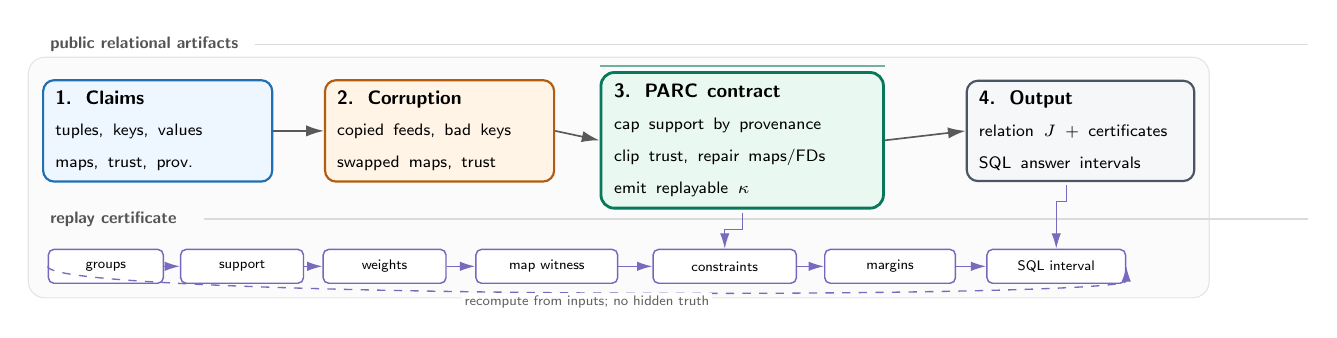
\begin{tikzpicture}[
  x=1cm,y=1cm,
  font=\sffamily,
  >=Latex,
  flow/.style={-{Latex[length=2.25mm,width=1.42mm]}, line width=.60pt, draw=black!65},
  replay/.style={-{Latex[length=1.95mm,width=1.20mm]}, line width=.48pt, draw=parcpurple!82},
  card/.style 2 args={draw=#1, fill=#2, rounded corners=4.0pt, line width=.78pt, align=left, inner xsep=4.4pt, inner ysep=3.8pt, minimum height=1.02cm, text width=2.60cm},
  core/.style={draw=parcgreen, fill=parcgreenbg, rounded corners=4.8pt, line width=1.02pt, align=left, inner xsep=4.8pt, inner ysep=4.2pt, minimum height=1.32cm, text width=3.25cm},
  output/.style={draw=parcslate, fill=parcslatebg, rounded corners=4.0pt, line width=.78pt, align=left, inner xsep=4.4pt, inner ysep=3.8pt, minimum height=1.02cm, text width=2.58cm},
  chip/.style={draw=parcpurple!84, fill=white, rounded corners=2.0pt, line width=.52pt, minimum height=.43cm, align=center, inner xsep=3.0pt, font=\sffamily\fontsize{5.25}{5.7}\selectfont},
  lane/.style={font=\sffamily\fontsize{5.95}{6.4}\selectfont\bfseries, text=black!67},
  tag/.style={font=\sffamily\fontsize{5.0}{5.5}\selectfont, fill=white, inner sep=.8pt, text=black!62},
]

\node[lane, anchor=west] at (0.10,3.02) {public relational artifacts};
\draw[black!14,line width=.50pt] (2.82,3.02) -- (16.20,3.02);

\node[card={parcblue}{parcbluebg}, anchor=west] (inp) at (0.12,1.92)
  {\boxtitle{1. Claims}\tightgap{-.2mm}\boxline{tuples, keys, values}\tightgap{-.15mm}\boxline{maps, trust, prov.}};
\node[card={parcorange}{parcorangebg}, anchor=west] (dirty) at (3.70,1.92)
  {\boxtitle{2. Corruption}\tightgap{-.2mm}\boxline{copied feeds, bad keys}\tightgap{-.15mm}\boxline{swapped maps, trust}};
\node[core, anchor=west] (parc) at (7.20,1.80)
  {\boxtitle{3. PARC contract}\tightgap{-.2mm}\boxline{cap support by provenance}\tightgap{-.15mm}\boxline{clip trust, repair maps/FDs}\tightgap{-.15mm}\boxline{emit replayable $\kappa$}};
\node[output, anchor=west] (out) at (11.85,1.92)
  {\boxtitle{4. Output}\tightgap{-.2mm}\boxline{relation $J$ + certificates}\tightgap{-.15mm}\boxline{SQL answer intervals}};

\draw[flow] (inp.east) -- (dirty.west);
\draw[flow] (dirty.east) -- (parc.west);
\draw[flow] (parc.east) -- (out.west);

\node[lane, anchor=west] at (0.10,.80) {replay certificate};
\draw[black!14,line width=.50pt] (2.18,.80) -- (16.20,.80);

\node[chip, minimum width=1.46cm] (c1) at (0.93,.20) {groups};
\node[chip, minimum width=1.56cm] (c2) at (2.66,.20) {support};
\node[chip, minimum width=1.56cm] (c3) at (4.47,.20) {weights};
\node[chip, minimum width=1.80cm] (c4) at (6.53,.20) {map witness};
\node[chip, minimum width=1.82cm] (c5) at (8.79,.20) {constraints};
\node[chip, minimum width=1.66cm] (c6) at (10.89,.20) {margins};
\node[chip, minimum width=1.76cm] (c7) at (13.00,.20) {SQL interval};
\foreach \a/\b in {c1/c2,c2/c3,c3/c4,c4/c5,c5/c6,c6/c7}{\draw[replay] (\a.east) -- (\b.west);}
\draw[replay] ($(parc.south)+(0,-.04)$) -- ++(0,-.21) -| (c5.north);
\draw[replay] ($(out.south)+(-.18,-.04)$) -- ++(0,-.21) -| (c7.north);
\draw[replay, dashed] (c1.west) .. controls +(0,-.42) and +(0,-.42) .. node[tag, below=.18mm] {recompute from inputs; no hidden truth} (c7.east);

\begin{scope}[on background layer]
  \node[draw=black!10, fill=black!1.5, rounded corners=6pt, fit=(inp)(dirty)(parc)(out)(c1)(c7), inner sep=5.0pt] {};
  \draw[parcgreen!58,line width=.75pt] ($(parc.north west)+(0,.07)$) -- ($(parc.north east)+(0,.07)$);
\end{scope}
\end{tikzpicture}
\end{document}
